\documentclass[12pt,a4paper,oneside]{book}
\usepackage{a4wide}                     % Iets meer tekst op een bladzijde
\usepackage[dutch,english]{babel}       % Voor nederlandstalige hyphenatie (woordsplitsing)
\usepackage{amsmath}                    % Uitgebreide wiskundige mogelijkheden
\usepackage{amssymb}                    % Voor speciale symbolen zoals de verzameling Z, R...
\usepackage{url}                        % Om url's te verwerken
\usepackage{graphicx}                   % Om figuren te kunnen verwerken
\usepackage[small,bf]{caption2}    % Om de captions wat te verbeteren
\usepackage{xspace}                     % Magische spaties na een commando
\usepackage[utf8]{inputenc}           	% Om niet ascii karakters rechtstreeks te kunnen typen
\usepackage{float}                      % Om nieuwe float environments aan te maken. Ook optie H!
\usepackage{flafter}                    % Opdat floats niet zouden voorsteken
\usepackage{listings}                   % Voor het weergeven van letterlijke text en codelistings
\usepackage{marvosym}                   % Om het euro symbool te krijgen
\usepackage{textcomp}                   % Voor onder andere graden celsius
\usepackage{fancyhdr}                   % Voor fancy headers en footers.
\usepackage{graphics}					% Om figuren te verwerken.
\usepackage[nottoc]{tocbibind} 			% Bibliografie in ToC; zie tocbibind.dvi
%\usepackage{pstricks}
\usepackage{longtable}
\usepackage{pdfpages}  					% pdf pagina's importeren
\usepackage[numbers]{natbib}			% Extra citeer mogelijkheden
\usepackage{parskip}					% Geen indentatie bij begin paragraaf
\usepackage[hang,flushmargin,bottom]{footmisc} % Voetnoten beter weergeven (niet laten splitsen)
\usepackage{enumitem} 					%Betere opsommingen
\usepackage{sidecap}  					%Caption lang
\usepackage[toc,page]{appendix} 		%Appendices toevoegen
\usepackage{tikz}						%Toevoegen van tikz figuren
\usepackage{pgfplots}					%Grafieken plotten in tikz figuren
\usepackage{wrapfig}					%Figuren wrappen
\interfootnotelinepenalty=10000

\newcommand{\npar}{\par \vspace{2.3ex plus 0.3ex minus 0.3ex} \noindent}	% Om witruimte te krijgen tussen paragrafen
\graphicspath{{figuren/}}               % De plaats waar latex zijn figuren gaat halen.
%\usepackage[bf]{caption2}				% Mooiere captions
\usepackage[a4paper,plainpages=false]{hyperref}    % Om hyperlinks te hebben in het pdfdocument.
\newcommand{\command}[1]{\lstinline[basicstyle=\tt]{#1}\xspace} %Voor commando's
\hyphenation{} 							% Splitsing van woorden

\renewcommand{\chaptermark}[1]{\markright{\MakeUppercase{#1}}}
\renewcommand{\sectionmark}[1]{\markright{\thesection~#1}}

\newcommand{\headerfmt}[1]{\textsl{\textsf{#1}}}
\newcommand{\headerfmtpage}[1]{\textsf{#1}}

\fancyhf{}
\fancyhead[LE,RO]{\headerfmtpage{\thepage}}
\fancyhead[LO]{\headerfmt{\rightmark}}
\fancyhead[RE]{\headerfmt{\leftmark}}
\renewcommand{\headrulewidth}{0.5pt}
\renewcommand{\footrulewidth}{0pt}

\fancypagestyle{plain}{ % eerste bladzijde van een hoofdstuk
	\fancyhf{}
	\fancyhead[LE,RO]{\headerfmtpage{\thepage}}
	\fancyhead[LO]{\headerfmt{\rightmark}}
	\fancyhead[RE]{\headerfmt{\leftmark}}
	\renewcommand{\headrulewidth}{0.5pt}
	\renewcommand{\footrulewidth}{0pt}
}

\renewcommand{\lstlistoflistings}{\begingroup
	\tocfile{\lstlistlistingname}{lol}
	\endgroup}


% anderhalve interlinie (opm: titelblad gaat uit van 1.5)
\renewcommand{\baselinestretch}{1.5}


%Pdf instellen, links, meta info
\hypersetup {
	pdfauthor = {Ward Van Assche},
	pdftitle = {Realtime signaal synchronisatie	met accoustic fingerprinting},
	pdfsubject = {Masterproef ingediend tot het behalen van de academische graad van Master of Science in de industriële wetenschappen: informatica, juni 2016},
	colorlinks = False,
%	pdfborder = {0 0 0}
}

%Titels wijzigen in correcte Nederlandse term
\renewcommand\lstlistlistingname{Lijst van codefragmenten}
\renewcommand\lstlistingname{Codefragment}
\addto{\captionsdutch}{\renewcommand{\bibname}{Referentielijst}}

\begin{document}
\selectlanguage{dutch}

% titelblad (voor kaft)
%  Titelblad

% Opmerking: gaat uit van een \baselinestretch waarde van 1.5 (die moet
% ingesteld worden voor het begin van de document environment)

\begin{titlepage}

\setlength{\hoffset}{-1in}
\setlength{\voffset}{-1in}
\setlength{\topmargin}{1.5cm}
\setlength{\headheight}{0.5cm}
\setlength{\headsep}{1cm}
\setlength{\oddsidemargin}{3cm}
\setlength{\evensidemargin}{3cm}
\setlength{\footskip}{1.5cm}
\enlargethispage{1cm}
% \textwidth en \textheight hier aanpassen blijkt niet te werken

\fontsize{12pt}{14pt}
\selectfont

\begin{center}


\includegraphics[height=2cm]{fig/ruglogo}

\vspace{0.5cm}

Faculteit Ingenieurswetenschappen en Architectuur\\
Vakgroep Informatietechnologie\\
Voorzitter: Prof.~Dr.~Ir.~Dani\"{e}l De Zutter

\vspace{3.5cm}

\fontseries{bx}
\fontsize{17.28pt}{21pt}
\selectfont

Realtime signaal synchronisatie \\
met accoustic fingerprinting

\fontseries{m}
\fontsize{12pt}{14pt}
\selectfont

\vspace{.6cm}

door 

\vspace{.4cm}

Ward Van Assche

\vspace{3.5cm}

Promotoren: Dr.~Marleen Denert, Joren Six\\
Scriptiebegeleider: Prof.~Helga Naessens\\

\vspace{2cm}

Masterproef ingediend tot het behalen van de academische graad van\\
Master of Science in de industri\"{e}le wetenschappen: informatica

\vspace{1cm}

Academiejaar 2015--2016

\end{center}
\end{titlepage}


% lege pagina (!!)

% titelblad (!!)

% geen paginanummering tot we aan de inhoudsopgave komen
\pagestyle{empty}

% voorwoord met dankwoord en toelating tot bruikleen (ondertekend)
%  Voorwoord (dankwoord) en toelating tot bruikleen

\newpage

\noindent \textbf{\huge Voorwoord}

\vspace{1.5cm}

\noindent

Zonder hulp van buitenaf zou ik er nooit in geslaagd zijn om mijn masterproef tot een goed einde te brengen. Daarom wil ik verschillende mensen bedanken die een grote rol gespeeld in één of meerdere fases van dit eindwerk.

Eerst en vooral wil ik mijn externe promotor, Joren Six, bedanken voor het vertrouwen en de ondersteuning die hij mij tijdens het uitwerken van deze masterproef heeft gegeven. De kennis en inzicht die ik van hem heb meegekregen op vlak van digitale audio (en alles wat ermee te maken heeft) zal mij zeker bijblijven. Ik vond het ontzettend leerrijk om mijn interesse in muziek en geluid te kunnen combineren met mijn opleiding informatica.

Verder wil ik ook mijn interne promotor, Marleen Denert, bedanken voor het opvolgen en nalezen van mijn thesis. Haar opbouwende kritiek was van onschatbare waarde.

Ten slotte wil ik ook mijn ouders, zusje en vrienden bedanken die mij altijd gesteund hebben tijdens mijn opleiding tot industrieel ingenieur.

En uiteraard wil ik ook u, de lezer, bedanken voor de interesse in mijn onderzoek. Ik wens u veel leesplezier.

\addvspace{2.5cm}

\noindent Ward Van Assche, juni 2016\newpage

\noindent \textbf{\huge Toelating tot bruikleen}

\vspace{1.5cm}

\noindent
``De auteur geeft de toelating deze scriptie voor consultatie beschikbaar
te stellen en delen van de scriptie te kopi\"eren voor persoonlijk
gebruik.\\
Elk ander gebruik valt onder de beperkingen van het auteursrecht,
in het bijzonder met betrekking tot de verplichting de bron uitdrukkelijk
te vermelden bij het aanhalen van resultaten uit deze scriptie.''

\addvspace{4cm}

\noindent Ward Van Assche, juni 2016


% overzicht
%  Overzichtsbladzijde met samenvatting

\newpage

{
\setlength{\baselineskip}{14pt}
\setlength{\parindent}{0pt}
\setlength{\parskip}{8pt}

\begin{center}

\noindent \textbf{\huge
Realtime signaal synchronisatie\\[8pt]
met accoustic fingerprinting
}

door 

Ward Van Assche

Masterproef ingediend tot het behalen van de academische graad van\\
Master of Science in de industriële wetenschappen: informatica

Academiejaar 2015--2016

Promotoren: Dr.~Marleen Denert, Joren Six\\
Scriptiebegeleider: Prof.~Helga Naessens

Faculteit Ingenieurswetenschappen en Architectuur\\
Universiteit Gent

Vakgroep Informatietechnologie\\
Voorzitter: Prof.~Dr.~Ir.~Dani\"{e}l De Zutter


\end{center}

\section*{Samenvatting}

% TODO: samenvatting schrijven

\textit{Todo: samenvatting schrijven}




\section*{Trefwoorden}

% TODO: trefwoorden

synchronisatie, realtime, datastromen, musicologie, accoustic fingerprinting

}
\newpage % strikt noodzakelijk om een header op deze blz. te vermijden


% abstract pdf toevoegen
\addcontentsline{toc}{chapter}{Extended abstract}
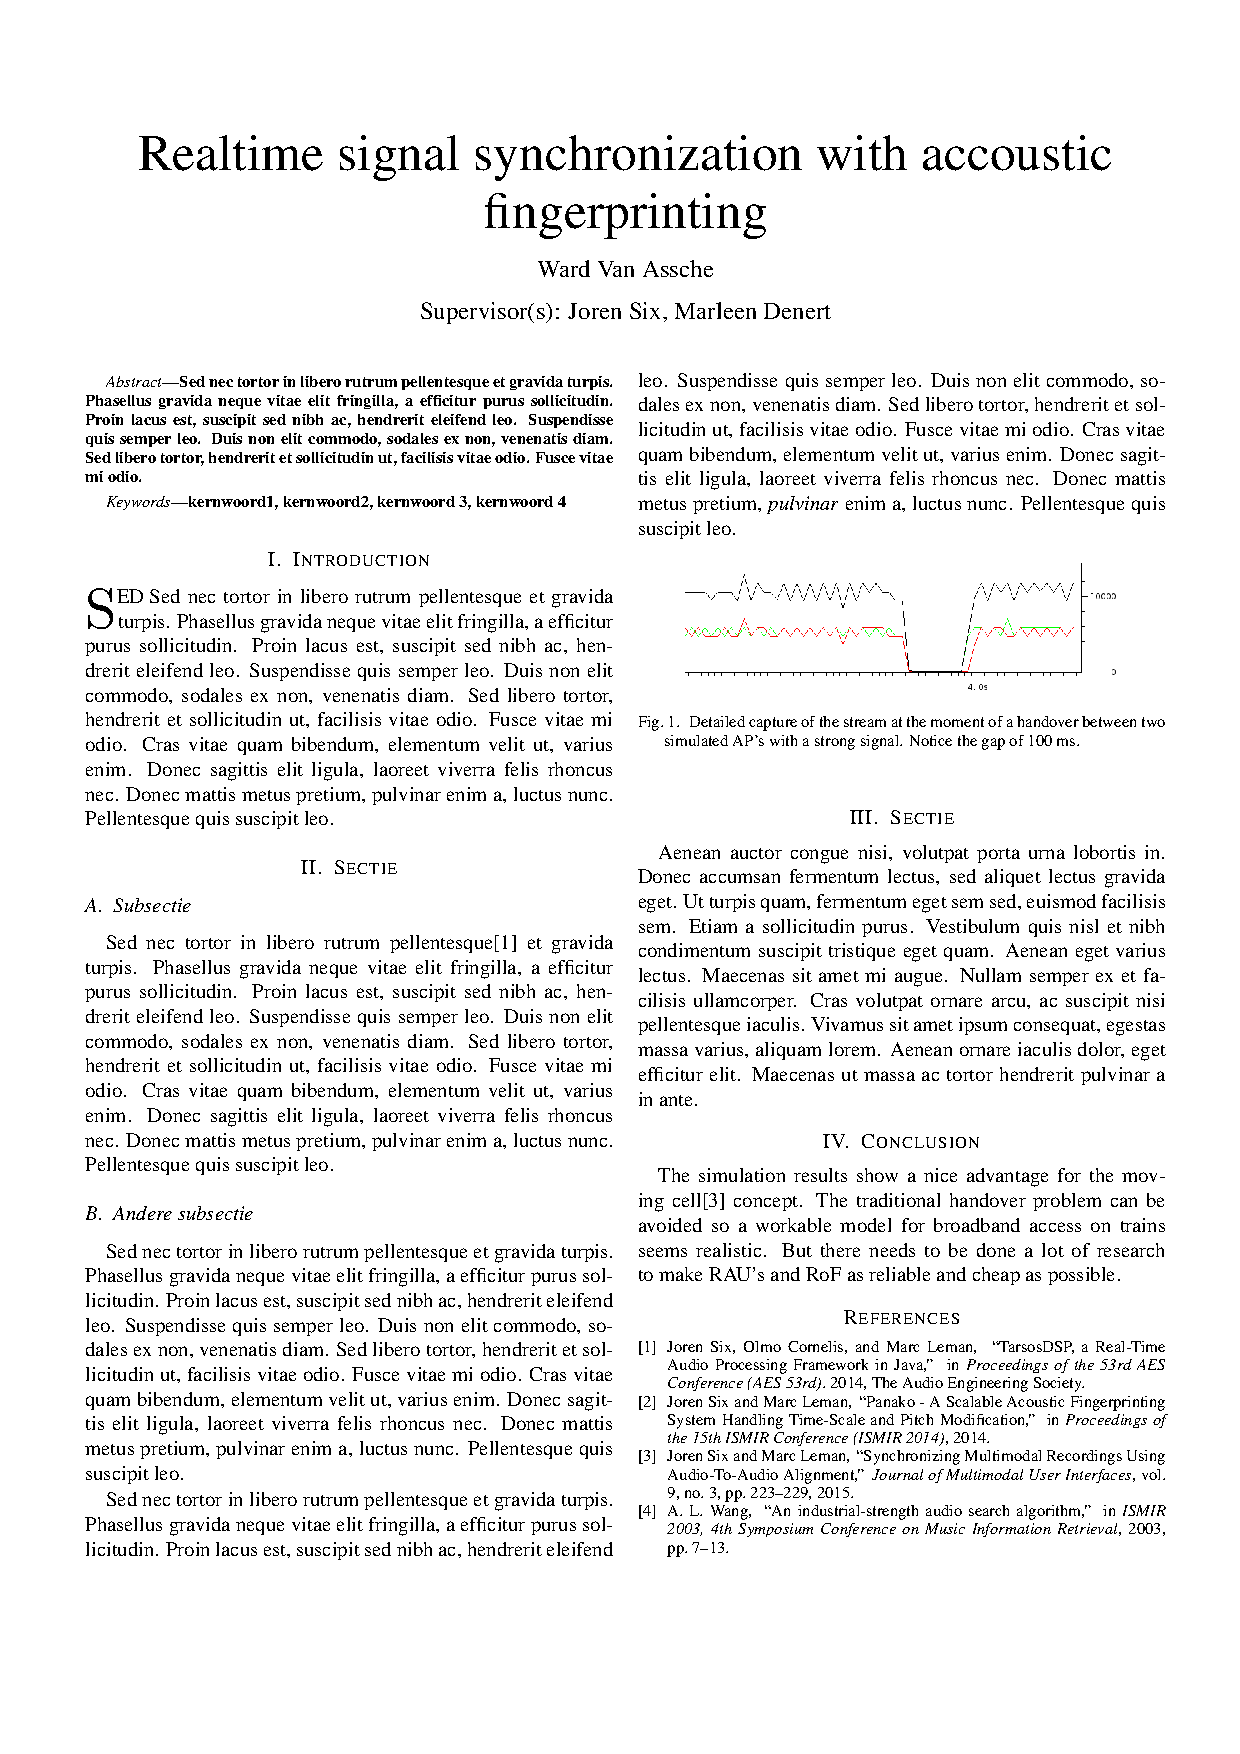
\includepdf[pages=-]{../abstract/abstract.pdf}
\pagestyle{fancy}

\frontmatter

% inhoudstafel
\tableofcontents

% afkortingen
\chapter{Gebruikte afkortingen}
\begin{flushleft}
	\renewcommand{\baselinestretch}{1.5}
	\small\normalsize
	\begin{longtable}{ll}
		IPEM				&  Instituut voor Psychoakoestiek en Elektronische Muziek \\
		DSP					&  Digital Signal Processing \\
		FFT					&  Fast Fourier Transform \\
		SFT					&  Short Time Fourier Transform \\
		ECG					&  Elektrocardiogram \\
		DTW					&  Dynamic timewarping \\
		USB					&  Universal Serial Bus \\
		ADC					&  Analog-to-digital converter \\
		PCM					&  Pulse-code modulation \\
		UML					&  Unified Modeling Language
		
	\end{longtable}
\end{flushleft}

% hoofdstukken
\mainmatter

% hier worden de hoofdstukken ingevoegd (\includes)
\chapter{Introductie}
\label{introductie}

\section{Probleemschets}
\label{probleemschets}

Het probleem dat in deze masterproef zal worden onderzocht doet zich heel specifiek voor bij verschillende experimenten die aan het IPEM worden uitgevoerd. Dit is de onderzoeksinstelling van het departement musicologie aan Universiteit Gent. De focus van het IPEM ligt vooral op onderzoek naar de interactie van muziek op fysieke aspecten van de mens zoals dansen, sporten en fysieke revalidatie. \cite{ipem2016}

Om de relatie tussen muziek en beweging te onderzoeken worden er tal van experimenten uitgevoerd. Deze experimenten maken gebruik van allerhande sensoren om bepaalde gebeurtenissen om te zetten in analyseerbare data. 

Bij een klassiek experiment wordt onderzocht wat de invloed is van muziek op de lichamelijke activiteit van een persoon. Alle bewegingen worden geregistreerd met een videocamera en een accelerometer.

Hierbij moeten drie datastreams worden geanalyseerd: de videobeelden, de data van de accelerometer en de afgespeelde audio. Een  uitdaging hierbij is de synchronisatie van deze verschillende datastreams. Om een goede analyse mogelijk te maken is het zeer gewenst dat men exact weet (tot op de milliseconde nauwkeurig) wanneer een bepaalde gebeurtenis in een datastream zich heeft voorgedaan, zodat men deze gebeurtenis kan vergelijken met de gebeurtenissen in de andere datastreams. Door de verschillen in samplefrequentie en door de latencies die zich in elke opname kunnen voordoen is dit zeker geen sinecure. \cite{six2015multimodal}

Bij het IPEM maakt men gebruik van een systeem waarbij audio opnames het synchronisatieproces vereenvoudigen. Het principe werkt als volgt: men zorgt ervoor dat elke datastream gekoppeld is aan een perfect gesynchroniseerde audiostream, afkomstig van een opname van het omgevingsgeluid. In het voorgaande experiment is dit eenvoudig te verwezenlijken. Bij de videobeelden kan automatisch een audiospoor mee worden opgenomen. De accelerometer kan geplaatst worden op een microcontroller vergezeld van een kleine microfoon. Aangezien beide componenten zo dicht op de hardware geplaatst zijn is de latency tussen beide datastromen te verwaarlozen.\footnote{De latency van de audioverwerking op een \textit{Axoloti} microcontroller is vastgesteld op $0.333 ms$. Meer informatie: \url{http://www.axoloti.com/more-info/latency/}} De afgespeelde audio is uiteraard al een perfecte weergave van het omgevingsgeluid. Figuur \ref{syncsink-ui} toont een screenshot van het programma waarmee de synchronisatie op dit moment wordt uitgevoerd.

Na het uitvoeren van het experiment beschikt men dus over de gegevens van drie datastreams, waarbij er aan elke datastream een quasi perfect synchrone opname van het omgevingsgeluid is gekoppeld. Aangezien het experiment in één ruimte is uitgevoerd zijn de verschillende opnames van het omgevingsgeluid zeer gelijkend. Het probleem van de synchronisatie van de verschillende datastromen kan bijgevolg gereduceerd worden tot het synchroniseren van de verschillende audiostromen.

Door de typisch eigenschappen van geluid is het niet zo moeilijk om verschillende audiostreams te synchroniseren. Bij het IPEM heeft men een systeem ontwikkeld dat hiertoe in staat is.

Dit systeem heeft in de praktijk echter heel wat beperkingen. De grootste beperking is dat het synchronisatieproces pas kan worden uitgevoerd wanneer het experiment is afgelopen. Deze verwerking kan ook enkel handmatig uitgevoerd worden. De opgenomen audio- en databestanden moeten worden verzameld op een computer waarna vervolgens de latency tussen de audiostreams bepaald kan worden. Met behulp van deze latency kunnen de datastreams worden gesynchroniseerd. 

Voor de musicologen die deze experimenten uitvoeren is deze werkwijze veel te omslachtig. Daarom is een eenvoudiger realtime systeem om de synchronisatie uit te voeren zeer gewenst.

\begin{figure}[!h]
	\captionsetup{width=0.7\textwidth}
	\centering
	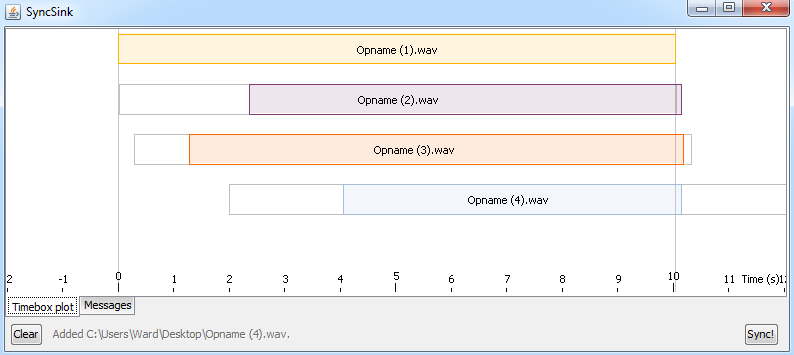
\includegraphics[width=0.5\textwidth]{syncsinc.png}
	\caption[Gebruikersinterface van SyncSink]{De gebruikersinterface van SyncSink: een programma waarin de opgenomen fragmenten gesleept kunnen worden na afloop van het experiment. Vervolgens wordt de latency berekend. Meer informatie is te vinden in artikel \cite{six2015multimodal}.}
	\label{syncsink-ui}
\end{figure}


Een ander probleem is dat de resultaten van het kruiscovariantie algoritme soms afwijkingen vertonen die moeilijk te verklaren zijn. De oorzaak hiervan zal worden onderzocht. Ook is het kruiscovariantie algoritme in vergelijking met het acoustic fingerprinting algoritme véél gevoeliger voor storingen en ruis, veroorzaakt door slechte opnames. Aangezien de opnameapparatuur (zeker op microcontrollers) bij de uit te voeren experimenten vaak van slechte kwaliteit is, is het belangrijk om de algoritmes voldoende robuust te maken zodat ze hier mee om kunnen.

\section{Digitale audio}

Het vervolg van deze scriptie onderstelt dat de lezer een basiskennis heeft inzake digitale audio. In deze inleiding worden de belangrijkste zaken hieromtrent uitgelegd.

Om geluidsgolven digitaal te kunnen verwerken moeten ze worden geconverteerd naar reeksen van discrete waarden. Deze omzetting gebeurt met een ADC: een analog-to-digital converter. De meeste ADC's maken gebruik van de PCM (pulse-code modulation) voorstelling van audio. Bij PCM wordt het analoge signaal op regelmatige tijdstippen gesampled en omgezet in discrete waarden. Figuur \ref{sampling} toont schematisch hoe dit in zijn werk gaat. PCM audio heeft verschillende parameters die een invloed hebben op de uiteindelijke kwaliteit van de audio. De belangrijkste parameters zijn de samplefrequentie (\textit{sampling rate}) en bitdiepte (\textit{bit depth}).

\begin{figure}[h!]
	\captionsetup{width=0.7\textwidth}
	\caption[Samplen van audio]{Samplen van een analoog audiosignaal in de vorm van een sinusgolf. Met toestemming overgenomen van artikel \cite{tarsosmanual2016}.}
	\begin{center}
		\advance\parskip0.3cm
		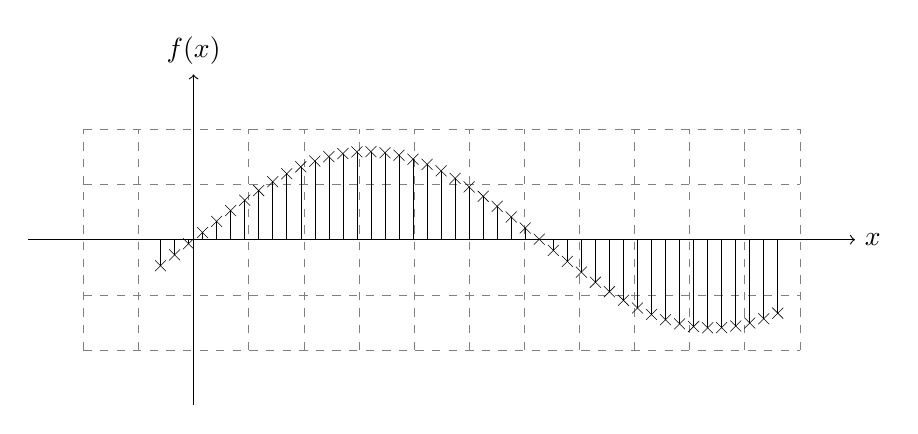
\begin{tikzpicture}[scale=1.4]
%grid
\draw[very thin,color=gray,step=.5cm,dashed] (-1,-1.0) grid (5.5,1);
\draw[->,color=black] (0,-1.5) -- (0,1.5)  node [above]{$f(x)$};
\draw[->,color=black] (-1.5,0) --  (6,0) node [right] {$x$};  
\draw[very thin,color=black,samples=45,domain=-0.3:5.3] 
plot[ycomb,thin,mark=x] (\x, { 0.8 * sin(\x r) });  
\end{tikzpicture}
	\end{center}
	\label{sampling}
\end{figure}

\subsubsection{Samplefrequentie}

De samplefrequentie bepaalt het aantal samples per seconde en wordt uitgedrukt in Hertz ($Hz$). Bij het bepalen van de samplefrequentie is het van belang om rekening te houden met het \textit{bemonsteringstheorema van Nyquist-Shannon}. Deze stelling zegt dat de samplefrequentie minstens dubbel zo hoog moet zijn dan de hoogste frequentie van de te converteren audio. Bij het samplen aan een lagere frequentie treedt informatieverlies op. Deze stelling wordt in detail besproken in het originele artikel \cite{nyquist1928certain} van \citeauthor{nyquist1928certain}.

Het menselijk oor is in staat om geluiden te detecteren tussen $20Hz$ en $20kHz$. Om informatieverlies bij het samplen van geluiden binnen dit bereik te voorkomen is het dus vereist om een minimale samplefrequentie te hanteren van $ 2 \times 20kHz $. De standaard samplefrequentie voor muziek is net iets hoger: $ 44.1kHz $.

De frequentie van de menselijke stem varieert tussen $ 30 Hz $ en $ 3000 Hz $. De minimale samplefrequentie voor het digitaliseren van een stemopname is dus $ 6kHz $. In de praktijk wordt meestal een minimum gehanteerd van $ 8kHz $.

\subsubsection{Bitdiepte}

De bitdiepte is het aantal bits waarmee elke gesamplede waarde wordt voorgesteld. Meestal wordt er gebruik gemaakt van 16 bit \textit{signed integers}.

De bitdiepte bepaalt het dynamische bereik van audio. Dit is de verhouding tussen het stilst en luidst mogelijk weer te geven volume. Deze verhouding, uitgedrukt in decibel, kan worden berekend met volgende formule: 
\begin{equation}
DR = 20 \cdot \log_{10} \left(\frac{2^Q}{1}\right) = (6.02 \cdot Q) dB
\end{equation}

In deze formule staat DR voor het dynamische bereik en Q voor de bitdiepte. Volgens deze formule heeft 16 bit audio een theoretisch dynamische bereik van ongeveer 96 dB. De werkelijke waarde kan hier echter van afwijken door filters die zijn ingebouwd in audiosystemen.

Bovenstaande informatie is gebaseerd op artikel \cite{tarsosmanual2016}, introductievideo \cite{xiph2016} en boek \cite{fries2005digital}.

\subsubsection{Weergave in software}

In computerprogramma's waarin digitale audio verwerkt wordt, wordt elke sample voorgesteld als een getal. Afhankelijk van de implementatie kan een 16 bit sample op verschillende manieren worden verwerkt. Enkele mogelijke voorstellingen: signed integer (-32768 tot 32767), unsigned integer (0 tot 65536) of floating point (-1 tot 1). 
In deze thesis en de bijhorende software wordt de floating point notatie gehanteerd.

\section{Evaluatiecriteria}
\label{evaluatie-criteria}

Het te ontwikkelen systeem moet voldoen aan heel wat vereisten. In deze sectie zullen de vereisten eenduidig geformuleerd en besproken worden.  

\subsubsection{Realtime synchronisatie}

Een cruciale vereiste is dat de toepassing in \textit{realtime} moet kunnen werken. Concreet wil dit zeggen dat de gesynchroniseerde data na het experiment onmiddellijk beschikbaar moet zijn.

Een écht realtime systeem bouwen is in de praktijk niet mogelijk. De algoritmes vereisen een bepaalde hoeveelheid aan data voordat de latency berekend kan worden. Daarom moeten de streams gebufferd worden, wat er toe leidt dat het systeem niet meer realtime is in de enge zin van het woord. Om een realtime systeem zo goed mogelijk te benaderen wordt een beperking opgelegd: een buffer met als maximumgrootte de hoeveelheid data verzameld in tien seconden. De buitengaande gesynchroniseerde streams hebben dus 10 seconden vertraging ten opzichte van de realtime streams.

\subsubsection{Detecteren van gedropte samples}

De beperkte resources van een microcontroller kan voor problemen zorgen bij het verwerken van streams. Zo kan het gebeuren dat er gegevens van streams verloren gaan. In het vakjargon worden dit ook wel \textit{gedropte samples} genoemd. Bij de synchronisatie leidt dit probleem tot een plotse verhoging van de latency. Hoewel het onmogelijk is om de gedropte samples te reconstrueren is het wel gewenst dat de gewijzigde latency gedetecteerd wordt en dat hiermee wordt rekening gehouden bij de verdere verwerking. De snelheid waarmee dit probleem gedetecteerd kan worden hangt eveneens af van de manier waarop er gebufferd wordt. Een detectiesnelheid van 10 seconden is aanvaardbaar voor deze toepassing.

\subsubsection{Detecteren van drift}

Elke stream heeft een eigen samplefrequentie. Het is belangrijk dat de samplefrequentie gekend is om de gegevens correct en precies te kunnen verwerken. Het kan echter voorvallen dat de samplefrequentie bij de verwerking op microcontrollers toch niet zo nauwkeurig bepaald is. Een stream waarbij de samplefrequentie $ 1Hz $ afwijkt van de theoretische waarde zal na 60 seconden een latency hebben opgebouwd van 60 samples. Bij een samplefrequentie van $8000 Hz$ komt dit overeen met $7.5 ms$.\footnote{Berekening: $ 60 / 8000 Hz = 0.0075 s = 7.5 ms $} Dit probleem mag zeker niet worden verwaarloosd. 

\section{Bestaande methoden}
\label{bestaande-methoden}

Er bestaan verschillende methoden om datastreams te synchroniseren. Welke methode te verkiezen is hangt volledig af van de toepassing.

In deze sectie komen de belangrijkste methoden aan bod en zullen ze worden getoetst aan de probleemstelling en de evaluatiecriteria.

\subsection{Event-gebaseerde synchronisatie}

Deze methode wordt beschreven in \cite{bannach2009automatic, six2015multimodal} en is een eenvoudige, vrij intuïtieve methode om synchronisatie van verschillende datastreams uit te voeren. De synchronisatie gebeurt aan de hand van markeringen die in de verschillende streams worden aangebracht. In audiostreams kan een kort en krachtig geluid een markering plaatsen. Een lichtflits kan dit realiseren in videostreams. De latency wordt bepaald door het verschil te berekenen tussen de tijdspositie van de markeringen in de streams. De synchronisatie kan vervolgens zowel manueel als softwarematig worden uitgevoerd.

Deze methode kent heel wat beperkingen. Zo vormt bij de synchronisatie van een groot aantal streams de schaalbaarheid een probleem. Ook wanneer er in een stream samples gedropt worden of er drift ontstaat, leidt dit tot foutieve synchronisatie. De methode kan deze twee problemen niet detecteren tot er opnieuw markeringen worden aangebracht en de streams gesynchroniseerd worden. Verder laten ook niet alle sensoren toe om markeringen aan te brengen: zo is de synchronisatie van een ECG onmogelijk met deze methode.

Het handmatig synchroniseren met behulp van deze methode blijkt derhalve in een realtime situatie niet mogelijk.  Wanneer de synchronisatie echter door software wordt uitgevoerd is deze methode wel in realtime bruikbaar. In dat geval moet er per tijdsinterval een markering worden aangebracht om de problemen veroorzaakt door drift en gedropte samples te overbruggen.

\subsection{Synchronisatie met een kloksignaal}

Artikel \cite{jaimovich2010synchronization} beschrijft een methode waarbij door een kloksignaal realtime streams van verschillende soorten toestellen worden gesynchroniseerd. Hiervoor gebruikt men standaard audio en video synchronisatieprotocollen. Elk toestel kan gebruik maken van verschillende samplefrequenties en communicatieprotocollen.

De methode gebruikt een \textit{master time code} signaal dat verstuurd wordt naar elk toestel. Dit laat het realtime analyseren van elke stream toe. Bij deze analyse kan vervolgens meteen de samplefrequentie en latency bepaald worden. 

Een groot nadeel van dit systeem is dat elk toestel een kloksignaal als input moet kunnen toelaten en verwerken. In het geval van de verwerking van videobeelden kan deze methode enkel gebruikt worden met zeer dure videocamera's waarbij de sluitertijd gecontroleerd kan worden. Bij goedkopere camera's (zoals's webcams) moet men op zoek gaan naar alternatieven. \cite{six2015multimodal}



\subsection{Dynamic timewarping}

Dynamic timewarping (DTW) is een techniek die gebruikt wordt voor het detecteren van gelijkenissen tussen twee tijdreeksen\footnote{Een tijdreeks is een sequentie van opeenvolgende datapunten over een continu tijdsinterval, waarbij de datapunten elk baar na telkens hetzelfde interval opvolgen.}. Aangezien een gedigitaliseerde audiostream een tijdreeks is kan deze techniek worden aangewend om de latency te bepalen tussen gelijkaardige opnames van het omgevingsgeluid. In de probleemschets (\ref{probleemschets}) is er uitgelegd hoe datastreams met behulp van het omgevingsgeluid gesynchroniseerd kunnen worden.

DTW is een algoritme dat op zoek gaat naar de meest optimale \textit{mapping} tussen twee tijdreeksen. Hierbij wordt gebruik gemaakt van een padkost. De padkost wordt bepaald door de manier waarop de tijdreeksen niet-lineair worden kromgetrokken ten opzichte van de tijdas\cite{salvador2007toward}. De minimale kost kan in kwadratische tijd berekend worden door gebruik te maken van dynamisch programmeren \cite{dixon2005live}. DTW is een veelgebruikte techniek in domeinen zoals spraakherkenning, bio-informatica, data-mining, etc \cite{ratanamahatana2004everything}.

Aangezien DTW het toelaat om tijdreeksen krom te trekken is het gewenst dat zowel het verleden als de toekomst van de streams voor het algoritme toegankelijk is. Een uitbreiding op dit algoritme beschreven in \cite{dixon2005live} laat toe één tijdreeks in realtime te streamen mits de andere stream op voorhand is gekend. Toch houdt deze uitbreiding geen oplossing in voor het gestelde probleem. Alle streams komen immers in realtime toe en de latency tussen de streams moet zo snel mogelijk achterhaald worden.

Het bufferen van de binnenkomende streams en vervolgens het DTW algoritme uit te voeren op de buffers leek een mogelijke manier om dit probleem te omzeilen.

Of het algoritme na deze aanpassing voldoet aan onze vereisten diende een klein experiment uit te wijzen. De resultaten hiervan zijn te vinden in appendix \ref{appendix-a}.

Het experiment toonde evenwel aan dat DTW niet bruikbaar is voor de realtime stream synchronisatie. De resultaten bleken niet nauwkeurig genoeg, zeker niet wanneer ook de performantie van het algoritme in beschouwing werd genomen.

\subsection{Acoustic fingerprinting}

Acoustic fingerprinting is een techniek die in staat is om gelijkenissen te vinden tussen verschillende audiofragmenten. Hierbij is het eveneens mogelijk om de latency tussen de audiofragmenten te bepalen. Net zoals bij DTW kan dit algoritme gebruikt worden om datastreams te synchroniseren met behulp van het omgevingsgeluid.

De techniek van acoustic fingerprinting extraheert en vergelijkt fingerprints van audiofragmenten. Een acoustic fingerprint bevat gecondenseerde informatie gebaseerd op typische eigenschappen van het audiofragment. De kracht van dit algoritme schuilt in haar snelheid en robuustheid. Het is immers uitzonderlijk bestand tegen achtergrondgeluiden en ruis. Door deze eigenschappen is het algoritme in staat om in enkele seconden een database met miljoenen fingerprints van audiofragmenten te doorzoeken. De bekendste toepassing van acoustic fingerprinting is de identificatie van liedjes op basis van een korte opname\footnote{Het grootste voorbeeld hiervan is de smartphone app Shazam. Deze app is de eerste toepassing dat gebruik maakte van dit algoritme.}.

Het is onder meer deze techniek die het IPEM gebruikt om de opgenomen audiostreams van experimenten te synchroniseren. In tegenstelling tot \textit{Shazam} wordt er niet op zoek gegaan naar matches in een database maar worden ze gezocht tussen de opgenomen audiofragmenten. Het uitgangspunt is immers dat er tussen de opnames gelijkenissen moeten gevonden kunnen worden.

Door haar snelheid en robuustheid lijkt dit algoritme te voldoen aan de vereisten om datastreams realtime te kunnen synchroniseren. Het is wel noodzakelijk dat de streams gebufferd worden alvorens het algoritme kan starten. Drift en gedropte samples kunnen gedetecteerd worden door het algoritme iteratief op korte gebufferde fragmenten uit te voeren. Na elke iteratie kan een eventuele wijziging worden opgemerkt. Zie \ref{acoustic-fingerprinting} voor een meer gedetailleerde bespreking van dit algoritme.

\subsection{Kruiscovariantie}

De laatste methode is net zoals de twee vorige methodes in staat om de latency tussen audiofragmenten te bepalen. Deze methode kan daarom ook aangewend worden om datastreams met behulp van opnames van het omgevingsgeluid te synchroniseren.

Kruiscovariantie (ook wel kruiscorrelatie genoemd) berekent de gelijkenis tussen twee audiofragmenten sample per sample en kent een getal toe aan de mate waarin de fragmenten overeenkomen. Door deze berekening voor elke verschuiving uit te voeren kan de latency tussen de fragmenten bepaald worden.

Deze methode is eveneens toepasbaar op realtime streams door gebruik te maken van buffering. Het iteratief uitvoeren van het algoritme op de opeenvolgende buffers zorgt ervoor dat gedropte samples en drift gedetecteerd kunnen worden.

In sectie \ref{kruiscovariantie} wordt dit algoritme verder in detail behandeld.

\section{Doel van deze masterproef}
\label{doel-masterproef}

Dit onderzoek wil drie zaken bereiken: 

\subsubsection{Selectie en optimalisatie van algoritmes}
Er wordt op zoek gegaan naar de algoritmes waarmee het probleem kan worden opgelost. Verder dienen de algoritmes en bijhorende parameters te worden geoptimaliseerd om in deze toepassing zo efficiënt mogelijk te presteren. Indien mogelijk zal er worden geprobeerd om de algoritmes waarvan er bij het IPEM al een implementatie beschikbaar is te hergebruiken.

Het beoogde doel is dat de algoritmes in staat zijn om audio opgenomen met een basic microfoon op een microcontroller te synchroniseren met een nauwkeurigheid van minstens één milliseconde.

\subsubsection{Ontwerp en implementatie van een softwarebibliotheek}
Het tweede doel van het onderzoek betreft het schrijven van een softwarebibliotheek. Deze bibliotheek zal gebruik maken van de geoptimaliseerde algoritmes om de latency tussen de verschillende audiostromen te bepalen. Deze bibliotheek moet vanuit andere software kunnen worden opgeroepen.

\subsubsection{Ontwerp en implementatie van een gebruiksvriendelijke interface}
\label{target-ui}

Uiteindelijk is het de bedoeling dat dit onderzoek resulteert in een gebruiksvriendelijke applicatie die toegankelijk is voor onderzoekers/musicologen zonder uitgebreide informatica kennis. De software moet in staat zijn om van verschillende datastreams (vergezeld van een audiostream) te synchroniseren en het gesynchroniseerde resultaat weg te schrijven naar een persistent medium.

\chapter{Methode}

\section{Algoritmen}

In sectie \ref{bestaande-methoden} van deze scriptie zijn de voornaamste methoden waarmee datastreams gesynchroniseerd kunnen worden beknopt besproken. Hoewel de meeste algoritmen niet voldeden aan de vereisten bleken er twee toch zeer geschikt voor snelle en nauwkeurige synchronisatie van realtime streams. In dit gedeelte zullen deze methoden in detail worden behandeld. Ook wordt er onderzocht in welke mate het mogelijk is om deze algoritmes te combineren tot één systeem.

\subsection{Accoustic fingerprinting}
\label{accoustic-fingerprinting}

Bij het accoustic fingerprinting algoritme worden fingerprints geëxtraheerd uit audiofragmenten. Het zoek naar gelijkenissen gebeurt door de fingerprints met elkaar te vergelijken. 

\subsubsection{Features}

Een cruciale stap bij de ontwikkeling van een accoustic fingerprinting systeem is het bepalen van een betrouwbare \textit{feature} om de fingerprints op te baseren. Een feature is een kenmerk waarmee het mogelijk is om audiofragmenten van elkaar te onderscheiden. Mogelijke features zijn bijvoorbeeld \textit{onsets}\footnote{Een onset is een markering in de tijd die het begin van een piek aanduidt. In artikel \cite{bello2005tutorial} wordt de betekenis en detectie van onsets uitgebreid beproken.} of frequentie. Een andere zeer goed bruikbare feature zijn de \textit{spectrale pieken} in het tijd-frequentie spectrum van de geluidsfragmenten. Deze feature is compact op te slaan en bevat veel informatie over het opgenomen audiofragment. Hierdoor wordt de kans kleiner dat fingerprints gematcht kunnen worden zonder dat ze daadwerkelijk gebaseerd zijn op hetzelfde geluid.

\begin{figure}[h!]
	\captionsetup{width=0.7\textwidth}
	\caption[Voorbeeld van een spectrogram]{Spectrogram van \textit{Talk Talk - New Grass}. De donkere vlekken zijn pieken zijn frequentie-intervallen die aan een relatief hoge energie voorkomen.}
	\begin{center}
		\advance\parskip0.3cm
		\begin{tikzpicture}
\begin{axis}[
xmin = 0,
xmax = 100,
ymin = 0,
ymax = 100,
ticks=none,
axis lines = left,
xlabel = Tijd,
ylabel = Frequentie,
width = 10.8cm,
height = 5.5cm
]
\addplot[thick,black] graphics[xmin=3,ymin=5,xmax=97,ymax=95] {talktalk.png};
\addplot+[mark = none] coordinates {};
\end{axis}
\end{tikzpicture}
	\end{center}
	\label{spectrogram}
\end{figure}

\subsubsection{Werking}

Een accoustic fingerprinting systeem gebaseerd op de extractie van spectrale pieken gaat in verschillende stappen te werk: 

Eerst wordt het tijdsignaal (de typische golfvorm) van elk geluidsfragment omgezet tot een verzameling functies in het frequentiedomein. Deze omzetting gebeurt met het \textit{Fast Fourier Transformation} algoritme (FFT). Het tijdsignaal wordt in kleine stukjes onderverdeeld (standaardgrootte: 512 samples, zie \ref{accoustic-fingerprinting-params}). Elk stukje audio wordt opgeslagen in een buffer waarop vervolgens het FFT algoritme op wordt uitgevoerd\footnote{Het uitvoeren van een FFT op zo'n klein stukje audio wordt ook wel de \textit{Short Time Fourier Transformation} of SFT genoemd}. De opeenvolgende buffers worden genummerd met een \textit{buffer index}. De inhoud van de buffer kan gezien worden als een signaal in het tijddomein. Het resultaat van het FFT algoritme is de fourier getransformeerde van dit signaal: een reeks van een eindig aantal frequentie-intervallen. Elke frequentie-interval is genummerd met een \textit{bin index}. De verzameling van alle fourier getransformeerden stelt het audiofragment voor in het tijd-frequentie domein. %Dit paragraaf nog eens laten nalezen

De grafische voorstelling van deze verzameling functies wordt het spectrogram genoemd. Een spectrogram is het duidelijkst wanneer op de x-as de tijd en op de y-as de frequentie wordt weergegeven. De intensiteit waarmee een bepaalde frequentie voorkomt kan worden aangeduid door gebruik te maken van verschillende kleuren of contrasten. Figuur \ref{spectrogram} toont een spectrogram waarbij frequentie met een hoge intensiteit donkerder zijn weergegeven.

In artikel \cite{oppenheim1970speech} wordt het FFT algoritme uitgebreid besproken.

Na het omzetten van de te vergelijken geluidsfragmenten naar hun tijd-frequentie representatie kan er naar kandidaat-pieken worden gezocht. Dit zijn lokale maxima waarbij de hoeveelheid energie waarmee de frequentie voorkomt hoger is dan bij zijn buren \cite{six2014panako}. In het spectrogram kan elk donker vlekje gezien worden als een kandidaat-piek.

Wanneer deze stap is afgerond kunnen de fingerprints bepaald worden. Een fingerprint is een de verbinding tussen twee spectrale pieken. Welke kandidaat-pieken gebruikt zullen worden in fingerprints hangt af van de implementatie van het algoritme en de ingestelde parameters. Enkele parameters die hier invloed op hebben zullen in sectie \ref{accoustic-fingerprinting-params} van deze scriptie besproken worden. Figuur \ref{kandidaat-pieken} toont een spectrogram met waarop enkele kandidaat-pieken en fingerprints zijn aangeduid.

\begin{figure}[h!]
	\captionsetup{width=0.7\textwidth}
	\caption[Kandidaat-pieken en fingerprints]{De kandidaat-pieken (gele stipjes) en fingerprints (rode lijnen)  van \textit{Talk Talk - New Grass}.}
	\begin{center}
		\advance\parskip0.3cm
		\begin{tikzpicture}
\begin{axis}[
xmin = 0,
xmax = 100,
ymin = 0,
ymax = 100,
ticks=none,
axis lines = left,
xlabel = Tijd,
ylabel = Frequentie,
width = 10.8cm,
height = 5.5cm
]
\addplot[thick,black] graphics[xmin=3,ymin=5,xmax=97,ymax=95] {talktalk-fingerprints.png};
\addplot+[mark = none] coordinates {};
\end{axis}
\end{tikzpicture}
	\end{center}
	\label{kandidaat-pieken}
\end{figure}

Na het bepalen van de fingerprints worden ze opgeslagen in een datastructuur waarin snel naar matches kan worden gezocht.
Om dit mogelijk te maken moeten er van de fingerprints enkele typerende getallen bepaald worden.

\begin{itemize}[noitemsep]
	\item $ f1 $ en $ f2 $: de frequentie van de spectrale pieken van de fingerprint.
	\item $ t1 $ en $ t2 $: de tijd van de spectrale pieken van de fingerprint.
	\item $ \Delta f $: het verschil van de frequenties van beide spectrale pieken van de fingerprint.
	\item $ \Delta t $: het verschil van de tijd van beide spectrale pieken van de fingerprint.
\end{itemize}

 Figuur \ref{schematische-fingerprint} toont een schematische voorstelling van een fingerprint waarop deze getallen zijn aangeduid.

\begin{figure}[h]
	\captionsetup{width=0.7\textwidth}
	\caption[De anatomie van een fingerprint]{De anatomie van een fingerprint in het tijd-frequentie domein. De rode lijn stelt de fingerprint voor tussen twee (niet afgebeelde) spectrale pieken. De typische parameters van de fingerprint zijn aangeduid op de assen. Met toestemming overgenomen uit artikel \cite{six2015multimodal}.}
	\begin{center}
		\advance\parskip0.3cm
		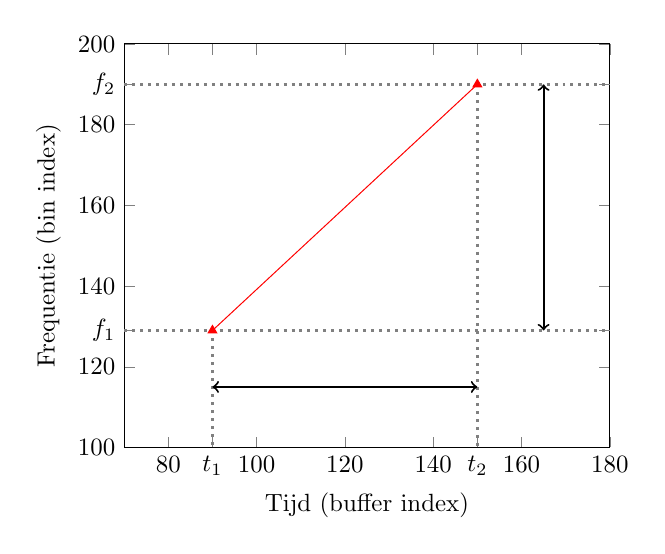
\begin{tikzpicture}[scale=0.9]
\begin{axis}[
	xlabel={Tijd (buffer index)},
	ylabel={Frequentie (bin index)},
	xmin=70,xmax=180,
	ymin=100,ymax=200,
	legend style={
  		cells={anchor=west},
  		legend pos=outer north east,
	},
	extra y ticks={129,190}, 
	extra y tick labels={$f_1$,$f_2$},
	extra x ticks={90,150}, 
	extra x tick labels={$t_1$,$t_2$},
]

  % plot the data from the file data.dat
  % smooth the curve and mark the data point with a dot
  \addplot[color=red,mark=triangle*] coordinates {
  	(90,129)
  	(150,190)
  };
  
  %f1
   \addplot[style= dotted,color=gray,very thick] coordinates{ (70,129)
   (180,129)};
   %f2
   \addplot[style= dotted,color=gray,very thick] coordinates{ (70,190)
   (180,190)};
   
    \node at (99,60) [] {\small$\Delta f$};
    \addplot[color=black,<->,thick] coordinates{ (165,129) (165,190)};
    
   \node at (50,18) [] {\small$\Delta t$};
   \addplot[style=dotted,color=gray,very thick] coordinates{ (90,129)
   (90,100)}; 
   \addplot[style=dotted,color=gray,very thick] coordinates{
   (150,190) (150,100)};
   \addplot[color=black,<->,thick] coordinates{ (90,115)
   (150,115)};
  
  \end{axis}
\end{tikzpicture}
	\end{center}
	\label{schematische-fingerprint}
\end{figure}

Bij het zoeken naar matches kan er gesteund worden op enkele typische eigenschappen van fingerprints: 

Twee overeenkomende fingerprints uit twee geluidsfragmenten zullen dezelfde frequenties  ($f1$ en $f2$) hebben. Bijgevolg is ook het verschil in frequentie ($\Delta f$) gelijk. 

De tijd van de spectrale pieken ($t1$ en $t2$) komen meestal niet overeen. Bij Shazam is het bijvoorbeeld geen vereiste om een opname te maken vanaf het begin van een liedje. Het moment van de opname mag volledig willekeurig worden gekozen. Bij het synchroniseren van streams wordt gezocht naar het verschil tussen de begintijden ($t1$ van elke fingerprint) van de overeenkomstige fingerprints van de audiofragmenten. Dit tijdverschil is wel gelijk bij elk paar overeenkomende fingerprints.

Hoewel de tijd ($t1$ en $t2$) van twee fingerprints meestal verschilt is dit niet het geval voor het verschil ervan ($\Delta t$). Bij twee overeenkomende fingerprints van twee audiofragmenten is het verschil in frequentie inherent gelijk.

Uit voorgaande eigenschappen kan geconcludeerd worden dat fingerprints uit twee audiofragmenten matchen wanneer $ f1 $, $ \Delta f $ en $ \Delta t $ gelijk zijn. Om deze parameters snel met elkaar kunnen te vergelijken wordt er een berekening uitgevoerd die deze parameters omzet in één enkel getal. Dit getal wordt de hash van de fingerprint genoemd. Samen met deze hash wordt ook $ t1 $ en een identificatie van het geluidsfragment bijgehouden.

Artikel \cite{six2014panako} geeft meer informatie over de omzetting van deze drie getallen tot een hash.

Een fingerprint kan bijgevolg gezien worden als verzameling gegevens met de volgende structuur: $ ( id; t1; hash(f1; \Delta f; \Delta t) ) $. Het zoeken naar fingerprints met overeenkomstige hashwaarden is mogelijk in $O(1)$ door gebruik te maken van een hashtabel. De precieze werking hiervan valt buiten de scope van deze scriptie.

Om te bepalen of twee audiofragmenten wel degelijk overeenkomen wordt er gezocht naar alle fingerprints met een overeenkomende hashwaarde. Van elk paar overeenkomende fingerprints wordt het verschil tussen $ t1 $ berekend. Dit verschil wordt de offset genoemd. Het vinden van een groot aantal matches met dezelfde offset wijst op een sterke gelijkenis tussen de audiofragmenten. De precieze waarde van ``een groot aantal'' wordt bepaald door een parameter van het algoritme.

\subsubsection{Bepalen van de latency}

Accoustic fingerprinting kan gebruikt worden om streams te synchroniseren door de ze eerst te bufferen. Wanneer een buffer volledig is opgevuld kan deze net zoals een kort audiofragment worden verwerkt door het algoritme. De latency tussen streams wordt bepaald door de offset die in vorig paragraaf werd beschreven: het verschil tussen de $ t1 $ waarden stelt namelijk de verschuiving tussen de geluidsfragmenten voor.

Figuur \ref{schematische-synchronisatie} toont schematisch alle stappen die moeten worden doorlopen om met behulp van accoustic fingerprinting audiostreams te synchroniseren.

\vspace{0.3cm}
\begin{figure}[h]
	\captionsetup{width=0.7\textwidth}
	\caption[Schema synchronisatie met fingerprinting]{Schematische voorstelling van synchronisatie met behulp van een accoustic fingerprinting systeem.}
	\advance\parskip0.5cm
	\begin{tikzpicture}[overlay]
\node at (-1,0) [minimum width=2cm] (A) {};

\node (rect) at (3,0) [draw,thin,minimum width=3cm,minimum height=1cm,align=center,font=\footnotesize] (B) {Feature \\[-0.7em] extractie};

\node (rect) at (8,0) [draw,thin,minimum width=3cm,minimum height=1cm,align=center,font=\footnotesize] (C) {Fingerprint \\[-0.7em] constructie};

\node (rect) at (13,-2) [draw,thin,minimum width=3cm,minimum height=1cm,align=center,font=\footnotesize] (G) {Andere \\[-0.7em] fingerprints};

\node (rect) at (13,0) [draw,thin,minimum width=3cm,minimum height=1cm,align=center,font=\footnotesize] (D) {Matchen en \\[-0.7em] bepalen latency};

\node at (17,0) [minimum width=2cm] (E) {};

\node at (0,-10) [minimum height=5cm] (F) {};

\draw [->] (A) -- (B) node [pos=0.4,above,align=center,font=\footnotesize] {Buffer};
\draw [->] (B) -- (C) node [pos=0.5,above,align=center,font=\footnotesize] {Features};
\draw [->] (C) -- (D) node [pos=0.5,above,align=center,font=\footnotesize] {Fingerprint};
\draw [->] (D) -- (E) node [pos=0.6,above,align=center,font=\footnotesize] {Latency};
\draw [->] (G) -- (D);

\end{tikzpicture}
	\advance\parskip1cm
	\label{schematische-synchronisatie}
\end{figure}
\vspace{2.5cm}

Een uitgebreidere beschrijving is te vinden in artikel \cite{Wang2003a}. De methode die in het artikel en deze scriptie besproken werd is beperkt tot het vergelijken van audiofragmenten die in tijd noch toonhoogte gewijzigd zijn. Aan het IPEM is een aangepaste methode ontwikkeld die dit wel toelaat \cite{six2014panako}.

\subsubsection{Nauwkeurigheid}

Zowel de snelheid waarmee wijzigingen van de latency bepaald kunnen worden als de nauwkeurigheid van de latency zelf hangt af van heel wat verschillende parameters van het algoritme.

De detectiesnelheid is vooral afhankelijk van de buffergrootte waarop het algoritme wordt uitgevoerd. Met deze instelling moet echter omzichtig worden omgegaan: een te kleine buffergrootte kan er toe leiden dat het algoritme niet meer in staat is om voldoende matches te vinden. Het kan helpen om andere parameters te wijzigen waardoor het vinden van een groot aantal matches gegarandeerd blijft. Deze parameters worden in sectie \ref{accoustic-fingerprinting-params} in detail besproken.

De nauwkeurigheid van de latency van het algoritme hangt af van de parameters van het FFT algoritme. Een nauwkeurigheid van 16 ms of 32 ms is standaard. De precieze werking van het FFT algoritme valt buiten de scope van deze scriptie.

\subsection{Kruiscovariantie}
\label{kruiscovariantie}

Deze methode bepaalt de gelijkenis tussen twee audiofragmenten en resulteert in één getal. Dit getal is een soort van score die aangeeft in welke mate twee signalen overeenkomen. De latency tussen twee audiofragmenten kan bepaald worden door deze berekening uit te voeren voor \textbf{elke mogelijke verschuiving}. De verschuiving waarbij het resulterend getal het hoogst is bepaalt de latency.

\subsubsection{Werking}

Stel twee audioblokken $ a $ en $ b $ bestaande uit een gelijk aantal samples ($n$). Deze audioblokken worden telkens cyclisch één sample verschoven tot wanneer de kruiscovariantie waarde ($ k $) voor elke mogelijke verschuiving berekend werd. De variabele $ i $ stelt de huidige verschuiving voor en gaat van 0 tot $ n $. De kruiscovariantie wordt berekend met formule:

\begin{equation}
	k = \sum_{j=0}^{n} a_{j} \cdot b_{(i+j)\ mod\ n}
\end{equation}

De waarde van $ i $ waarbij de kruiscovariantie het hoogst is stelt de latency voor tussen beide audioblokken in aantal samples. De latency in seconden kan bepaald worden door dit resultaat te delen door de samplefrequentie.

De methode kan de latency \textbf{tot op één sample nauwkeurig} bepalen. De maximaal bereikbare nauwkeurigheid hangt dus af van de samplefrequentie van de audioblokken. Bij een samplefrequentie van $8000 Hz$ is dit $ 1/8000 Hz = 0.125 ms $. Dit is ruim voldoende voor het huidige probleem.

Een nadeel aan deze methode is de performantie. Het berekenen van de beste kruiscovariantie van twee audioblokken bestaande uit $ n $ samples kan gebeuren in  $O(n^{2})$. Het is dus belangrijk om bij deze berekening de grootte van de audioblokken te beperken.

In artikel \cite{six2015multimodal} wordt deze techniek meer in detail besproken.

\subsubsection{Toepassing in realtime}

Het bufferen van de audiostreams maakt ook dit algoritme in realtime toepasbaar. In tegenstelling tot accoustic fingerprinting is het niet de bedoeling dat de berekeningen op de volledige buffer wordt uitgevoerd. Door de kwadratische tijdscomplexiteit zou het algoritme onnoemelijk veel rekenkracht vragen.\footnote{Voor het berekenen van de kruiscovariantie tussen twee buffers met $10s$ audio en een samplefrequentie van $8000hz$ zijn er asymptotisch $ 6.4 \cdot 10^9 $ berekeningen vereist.} Er moet dus een manier gevonden worden waarmee het mogelijk is om het aantal samples waarop het algoritme wordt uitgevoerd beperkt wordt.

\subsection{Toepasbaarheid}
\label{toepasbaarheid}

Het accoustic fingerprinting algoritme is zeer snel en robuust en kan gebruikt worden om gebufferde audiostreams te synchroniseren tot enkele tientallen milliseconden nauwkeurig (afhankelijk van de parameters van het FFT algoritme).

Het kruiscovariantie algoritme kan eveneens gebruikt worden om (gebufferde) audiostreams te synchroniseren. De grootste troef van dit algoritme is haar nauwkeurigheid: in de beste omstandigheden kan het algoritme resultaten bekomen tot op één sample nauwkeurig. Het bereiken van een dergelijke nauwkeurigheid is onmogelijk met eender welk ander besproken algoritme. De keerzijde is de performantie van het algoritme. Bij het synchroniseren van grote audioblokken kan dit problematisch zijn.

De kenmerken van deze algoritmen zijn complementair. De gemakkelijkste manier om een robuust, snel én nauwkeurig systeem op te bouwen is door het beste van de twee werelden te combineren. Het accoustic fingerprinting algoritme kan zorgen voor de synchronisatie tot op enkele tientallen milliseconden nauwkeurig. Dit resultaat laat toe dat we het kruiscovariantie algoritme kunnen uitvoeren op zeer korte stukjes audio (een honderdtal milliseconden volstaat).

\section{Bufferen van streams}
\label{streambuffers}

Aangezien de algoritmes een bepaalde hoeveelheid audio nodig hebben vooraleer ze kunnen worden uitgevoerd is het noodzakelijk om de streams eerst te bufferen. Dit proces moet herhaald worden aangezien er mogelijk samples gedropt worden of drift kan ontstaan. In dit deel zal worden uitgelegd hoe het bufferen precies in zijn werk gaat. Om verwarring met andere soorten buffers te vermijden zal dit type buffer verder in deze scriptie een \textit{streambuffer} genoemd worden.

\subsubsection{Buffergrootte}

De grootte van de buffer heeft invloed op de kwaliteit van de resultaten. Het spreekt voor zich dat het algoritme beter kan presteren wanneer er 10 seconden in plaats van 1 seconde audio geanalyseerd wordt. Een nadeel is echter dat het langer duurt vooraleer een wijzing van de latency gedetecteerd kan worden. 

\subsubsection{Naïeve implementatie}

Indien er buffers gebruikt worden die $ t $ aantal seconden audio kunnen bevatten, dan zal het bij een naïeve implementatie in het slechtste geval pas mogelijk zijn om een wijziging van de latency na $ \frac{3}{2} t $ seconden te detecteren. Dit is als volgt te verklaren: Een wijziging van de latency kan gedetecteerd worden wanneer meer dan de helft van de buffer gevuld is met audio met de nieuwe latency. Wanneer er samples gedropt worden net na het moment dat de buffer voor de helft gevuld is ($ \frac{1}{2} t $), dan zal het algoritme uitgevoerd op de huidige buffer de wijziging niet kunnen detecteren. De volgende buffer zal wel gevuld zijn audio met de nieuwe latency, het duurt echter nog een bijkomende $ t $ seconden vooraleer deze buffer gevuld is. De detectietijd bedraagt bijgevolg in het slechtste geval dus $ \frac{3}{2} t $ seconden.

De naïeve implementatie kan een wijziging van de latency in het beste geval na $ \frac{1}{2} t $ seconden detecteren. Wanneer er samples gedropt worden net voor het moment dat de buffer voor de helft gevuld is, dan kan het algoritme de nieuwe latency wel onmiddellijk detecteren.

\subsubsection{Sliding window}

Een meer doordachte manier van bufferen maakt gebruik van een \textit{sliding window}. In onderstaande beschrijving wordt gebruik gemaakt van een buffer met $ t $ seconden capaciteit en een stapgrootte van $ s $ seconden, hierbij geldt dat $ s \leq t $. 

Het verschil met de naïeve methode is dat de buffer niet pas na $ t $ seconden wordt opgeschoven. Door de buffer al na $ s $ seconden op te schuiven zal een wijziging van de latency sneller gedetecteerd kunnen worden; dit terwijl het algoritme toch nog steeds $ s $ seconden audio kan analyseren. In figuur \ref{slidingwindow} wordt grafisch weergegeven hoe de buffer precies verschoven wordt met $ t = 10 $ en $ s = 5 $.

\begin{figure}[h!]
	\captionsetup{width=0.7\textwidth}
	\caption[Schematische weergave van de buffer]{Schematische weergave van een \textit{sliding window} buffer over een audiostream.}
	\begin{center}
		\advance\parskip0.3cm
		\begin{tikzpicture}[scale=0.9]
\begin{axis}[
xlabel={Tijd (seconden)},
xmin=170,xmax=200,
ymin=0,ymax=1,
legend style={
	cells={anchor=west},
	legend pos=outer north east,
},
yticklabels={,,},
xticklabel style={grid=major},
extra x ticks={176,177,186,187},
extra x tick labels={,,,},
extra tick style={grid=major, grid style={dotted}},
hide y axis
]
\addplot[thick,black] graphics[xmin=140,ymin=0,xmax=200,ymax=1] {wave.png};

after end axis/.code={
	\draw[black,<->] (axis cs:175,0.1) -- (axis cs:185,0.1)	node [pos=0.5,above,font=\scriptsize] {buffer $i-1$};
	
	\draw[black,<->] (axis cs:176,0.2) -- (axis cs:186,0.2)	node [pos=0.5,above,font=\scriptsize] {buffer $i$};
	
	\draw[black,<->] (axis cs:177,0.3) -- (axis cs:187,0.3)	node [pos=0.5,above,font=\scriptsize] {buffer $i+1$};
}]

%\node at (50,18) [] {\small$\Delta t$};
%\addplot[style=dotted,color=gray,very thick] coordinates{ (90,129)
%	(90,100)}; 
%\addplot[style=dotted,color=gray,very thick] coordinates{
%	(150,190) (150,100)};
%\addplot[color=black,<->,thick] coordinates{ (90,115)
%	(150,115)};

\end{axis}

\end{tikzpicture}
	\end{center}
	\label{slidingwindow}
\end{figure}

Door de buffer al na $ s $ seconden op te schuiven wordt het slechtste geval sterk verbeterd. In het slechtste geval wordt een wijziging van de latency gedetecteerd na $ \frac{t}{2} + s $ seconden. Het beste geval blijft wel nog steeds $ \frac{t}{2} $ seconden.

Het verkleinen van de stapgrootte zorgt ervoor dat het algoritme per hoeveelheid audio frequenter moet worden uitgevoerd. Een te kleine stapgrootte heeft bijgevolg een negatieve invloed op de performantie.

\subsubsection{Voorbeeld}

Een praktisch voorbeeld zal bovenstaande beschrijving wat verduidelijken. In het voorbeeld worden twee audiostreams van 40 seconden geanalyseerd. Door het droppen van samples neemt de latency tussen de streams stapsgewijs toe. Figuur \ref{latency} toont in het zwart hoe de latency gedurende de verwerking evolueert. De opeenvolgende buffers van de twee besproken methode's worden in het rood aangeduid. 

\begin{figure}[h!]
	\captionsetup{width=0.7\textwidth}
	\caption[Voorbeeld buffering methodes]{Grafisch weergave van de methode's waarop gebufferd kan worden. De zwarte lijn stelt de huidige latency voor. In het rood worden de opeenvolgende buffers weergegeven.}
	\begin{center}
		\advance\parskip0.3cm
		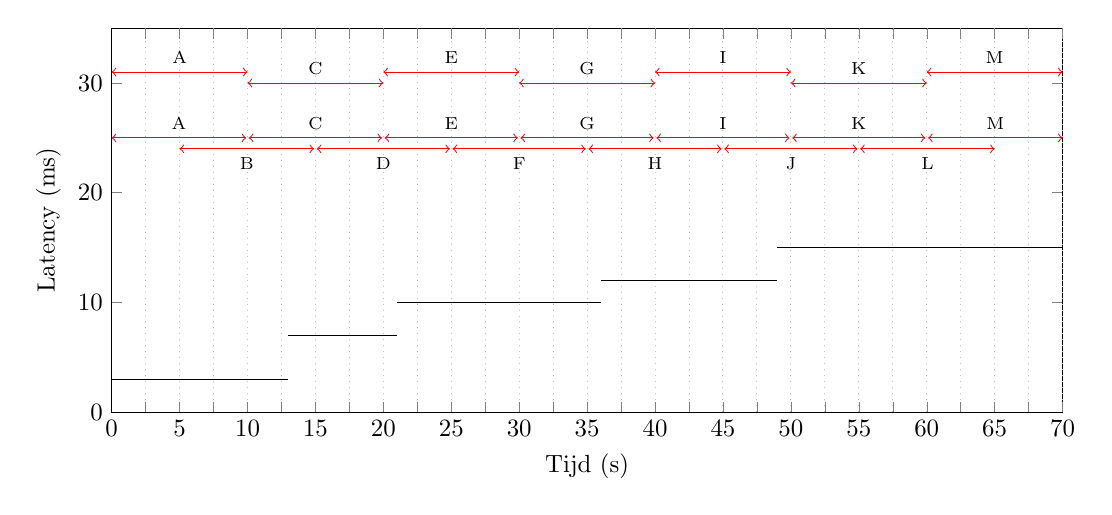
\begin{tikzpicture}[scale=0.9]
\begin{axis}[
xlabel={Tijd (s)},
ylabel={Latency (ms)},
xmin=0,xmax=70,
ymin=0,ymax=35,
legend style={
	cells={anchor=west},
	legend pos=outer north east,
},
extra x ticks ={2.5,5,7.5,...,70},
extra x tick labels={,,,},
extra x tick style={grid=major, grid style={dotted}},
width = 15cm,
height = 7cm
]



after end axis/.code={
	\draw (axis cs:0,3) -- (axis cs:13,3);
	\draw (axis cs:13,7) -- (axis cs:21,7);
	\draw (axis cs:21,10) -- (axis cs:36,10);
	\draw (axis cs:36,12) -- (axis cs:49,12);
	\draw (axis cs:49,15) -- (axis cs:70,15);
	
	\draw[red,<->] (axis cs:0,31) -- (axis cs:10,31)	node [pos=0.5,above,font=\scriptsize,color=black] {A};
	\draw[red,<->] (axis cs:10,30) -- (axis cs:20,30)	node [pos=0.5,above,font=\scriptsize,color=black] {C};
	\draw[red,<->] (axis cs:20,31) -- (axis cs:30,31)	node [pos=0.5,above,font=\scriptsize,color=black] {E};
	\draw[red,<->] (axis cs:30,30) -- (axis cs:40,30)	node [pos=0.5,above,font=\scriptsize,color=black] {G};
	\draw[red,<->] (axis cs:40,31) -- (axis cs:50,31)	node [pos=0.5,above,font=\scriptsize,color=black] {I};
	\draw[red,<->] (axis cs:50,30) -- (axis cs:60,30)	node [pos=0.5,above,font=\scriptsize,color=black] {K};
	\draw[red,<->] (axis cs:60,31) -- (axis cs:70,31)	node [pos=0.5,above,font=\scriptsize,color=black] {M};
	
	\draw[red,<->] (axis cs:0,25) -- (axis cs:9.9,25)	node [pos=0.5,above,font=\scriptsize,color=black] {A};
	\draw[red,<->] (axis cs:5,24) -- (axis cs:14.9,24)	node [pos=0.5,below,font=\scriptsize,color=black] {B};
	\draw[red,<->] (axis cs:10.1,25) -- (axis cs:19.9,25)	node [pos=0.5,above,font=\scriptsize,color=black] {C};
	\draw[red,<->] (axis cs:15.1,24) -- (axis cs:24.9,24)	node [pos=0.5,below,font=\scriptsize,color=black] {D};
	\draw[red,<->] (axis cs:20.1,25) -- (axis cs:29.9,25)	node [pos=0.5,above,font=\scriptsize,color=black] {E};
	\draw[red,<->] (axis cs:25.1,24) -- (axis cs:34.9,24)	node [pos=0.5,below,font=\scriptsize,color=black] {F};
	\draw[red,<->] (axis cs:30.1,25) -- (axis cs:39.9,25)	node [pos=0.5,above,font=\scriptsize,color=black] {G};
	\draw[red,<->] (axis cs:35.1,24) -- (axis cs:44.9,24)	node [pos=0.5,below,font=\scriptsize,color=black] {H};
	\draw[red,<->] (axis cs:40.1,25) -- (axis cs:49.9,25)	node [pos=0.5,above,font=\scriptsize,color=black] {I};
	\draw[red,<->] (axis cs:45.1,24) -- (axis cs:54.9,24)	node [pos=0.5,below,font=\scriptsize,color=black] {J};
	\draw[red,<->] (axis cs:50.1,25) -- (axis cs:59.9,25)	node [pos=0.5,above,font=\scriptsize,color=black] {K};
	\draw[red,<->] (axis cs:55.1,24) -- (axis cs:65,24)	node [pos=0.5,below,font=\scriptsize,color=black] {L};
	\draw[red,<->] (axis cs:60.1,25) -- (axis cs:70,25)	node [pos=0.5,above,font=\scriptsize,color=black] {M};
	
%	\draw[black,<->] (axis cs:10,0.2) -- (axis cs:20,0.2)	node [pos=0.5,above,font=\scriptsize] {buffer $i$};
	
%	\draw[black,<->] (axis cs:20,0.3) -- (axis cs:30,0.3)	node [pos=0.5,above,font=\scriptsize] {buffer $i+1$};
}]

\end{axis}

\end{tikzpicture}
	\end{center}
	\label{latency}
\end{figure}

De initiële latency van 3 milliseconden wordt zowel met de naïeve methode als met het sliding window gedetecteerd na de analyse van de allereerste buffer (A of R) 10 seconden na aanvang van de analyse. De eerste verhoging tot 7 milliseconden vindt te laat plaats om gedetecteerd te kunnen worden door de eerste buffer van beide methodes. Bij deze verhoging van de latency wordt het verschil tussen beide methodes zichtbaar: bij  de sliding window methode vindt de detectie 6 seconden na de wijziging plaats. Bij de naïeve methode moet er echter gewacht worden tot wanneer buffer B is volgelopen 12 seconden na de wijziging. De tweede verhoging naar 10 seconden wordt zowel door de naïeve methode als door de sliding window methode gedetecteerd na 8 seconden (buffer C of W). De laatste wijziging naar 12 seconden kan door de naïeve methode pas gedetecteerd worden na 14 seconden (de buffer is niet meer zichtbaar op de grafiek). De sliding window methode zal deze wijziging na 6 seconden detecteren.

\subsubsection{Conclusie}

De detectiesnelheid van een latencywijziging hangt af van twee parameters: de bufferlengte ($t$) en de staplengte ($s$). Het beste geval ($ T_b $) heeft volgende ondergrens:
\begin{equation}
T_b = \frac{t}{2}
\end{equation}

Bij het slechtste geval ($ T_s $) moet ook rekening gehouden worden met de stapgrootte. De bovengrens wordt als volgt bepaalt:
\begin{equation}
T_s = \frac{t}{2} + s
\end{equation}

Bij het toepassen van deze formules op het voorbeeld uit het vorige paragraaf kan er worden vastgesteld dat in het beste geval een latencywijziging gedetecteerd kan worden na 5 seconden. In het slechtste geval wordt een dergelijke wijziging bij de naïeve methode ($t = s = 10 $) pas gedetecteerd na 15 seconden. Bij de sliding window methode ($t = 10, s = 4 $) is deze wachttijd echter begrensd tot maximaal 9 seconden.

%Evaluatiecriteria
\chapter{Evaluatie}
\label{evaluatie}

%Lorem ipsum dolor sit amet, consectetur adipiscing elit. Maecenas at facilisis diam, vel varius mi. Maecenas in sodales tellus. Aenean tincidunt erat sit amet accumsan bibendum. Aliquam posuere dictum diam in tempor. Aenean feugiat eget quam id malesuada. Proin pretium et urna mattis molestie. Mauris pretium neque id magna sodales pulvinar. Cum sociis natoque penatibus et magnis dis parturient montes, nascetur ridiculus mus. Sed vel ornare leo. Nullam porttitor diam eget blandit hendrerit.


\section{Unit testen}

%Lorem ipsum dolor sit amet, consectetur adipiscing elit. Maecenas at facilisis diam, vel varius mi. Maecenas in sodales tellus. Aenean tincidunt erat sit amet accumsan bibendum. Aliquam posuere dictum diam in tempor. Aenean feugiat eget quam id malesuada. Proin pretium et urna mattis molestie. Mauris pretium neque id magna sodales pulvinar. Cum sociis natoque penatibus et magnis dis parturient montes, nascetur ridiculus mus. Sed vel ornare leo. Nullam porttitor diam eget blandit hendrerit.


\section{Stresstesten}

%Lorem ipsum dolor sit amet, consectetur adipiscing elit. Maecenas at facilisis diam, vel varius mi. Maecenas in sodales tellus. Aenean tincidunt erat sit amet accumsan bibendum. Aliquam posuere dictum diam in tempor. Aenean feugiat eget quam id malesuada. Proin pretium et urna mattis molestie. Mauris pretium neque id magna sodales pulvinar. Cum sociis natoque penatibus et magnis dis parturient montes, nascetur ridiculus mus. Sed vel ornare leo. Nullam porttitor diam eget blandit hendrerit.


\section{Test in de praktijk}

%Lorem ipsum dolor sit amet, consectetur adipiscing elit. Maecenas at facilisis diam, vel varius mi. Maecenas in sodales tellus. Aenean tincidunt erat sit amet accumsan bibendum. Aliquam posuere dictum diam in tempor. Aenean feugiat eget quam id malesuada. Proin pretium et urna mattis molestie. Mauris pretium neque id magna sodales pulvinar. Cum sociis natoque penatibus et magnis dis parturient montes, nascetur ridiculus mus. Sed vel ornare leo. Nullam porttitor diam eget blandit hendrerit.


\section{Usability testen}

%Lorem ipsum dolor sit amet, consectetur adipiscing elit. Maecenas at facilisis diam, vel varius mi. Maecenas in sodales tellus. Aenean tincidunt erat sit amet accumsan bibendum. Aliquam posuere dictum diam in tempor. Aenean feugiat eget quam id malesuada. Proin pretium et urna mattis molestie. Mauris pretium neque id magna sodales pulvinar. Cum sociis natoque penatibus et magnis dis parturient montes, nascetur ridiculus mus. Sed vel ornare leo. Nullam porttitor diam eget blandit hendrerit.


\section{Analyse van de complexiteitsgraad}

%Lorem ipsum dolor sit amet, consectetur adipiscing elit. Maecenas at facilisis diam, vel varius mi. Maecenas in sodales tellus. Aenean tincidunt erat sit amet accumsan bibendum. Aliquam posuere dictum diam in tempor. Aenean feugiat eget quam id malesuada. Proin pretium et urna mattis molestie. Mauris pretium neque id magna sodales pulvinar. Cum sociis natoque penatibus et magnis dis parturient montes, nascetur ridiculus mus. Sed vel ornare leo. Nullam porttitor diam eget blandit hendrerit.


\section{Praktische bruikbaarheid van het systeem}

%Lorem ipsum dolor sit amet, consectetur adipiscing elit. Maecenas at facilisis diam, vel varius mi. Maecenas in sodales tellus. Aenean tincidunt erat sit amet accumsan bibendum. Aliquam posuere dictum diam in tempor. Aenean feugiat eget quam id malesuada. Proin pretium et urna mattis molestie. Mauris pretium neque id magna sodales pulvinar. Cum sociis natoque penatibus et magnis dis parturient montes, nascetur ridiculus mus. Sed vel ornare leo. Nullam porttitor diam eget blandit hendrerit.

\chapter{Conclusie}

%Lorem ipsum dolor sit amet, consectetur adipiscing elit. Maecenas at facilisis diam, vel varius mi. Maecenas in sodales tellus. Aenean tincidunt erat sit amet accumsan bibendum. Aliquam posuere dictum diam in tempor. Aenean feugiat eget quam id malesuada. Proin pretium et urna mattis molestie. Mauris pretium neque id magna sodales pulvinar. Cum sociis natoque penatibus et magnis dis parturient montes, nascetur ridiculus mus. Sed vel ornare leo. Nullam porttitor diam eget blandit hendrerit.

%Lorem ipsum dolor sit amet, consectetur adipiscing elit. Maecenas at facilisis diam, vel varius mi. Maecenas in sodales tellus. Aenean tincidunt erat sit amet accumsan bibendum. Aliquam posuere dictum diam in tempor. Aenean feugiat eget quam id malesuada. Proin pretium et urna mattis molestie. Mauris pretium neque id magna sodales pulvinar. Cum sociis natoque penatibus et magnis dis parturient montes, nascetur ridiculus mus. Sed vel ornare leo. Nullam porttitor diam eget blandit hendrerit.

%Lorem ipsum dolor sit amet, consectetur adipiscing elit. Maecenas at facilisis diam, vel varius mi. Maecenas in sodales tellus. Aenean tincidunt erat sit amet accumsan bibendum. Aliquam posuere dictum diam in tempor. Aenean feugiat eget quam id malesuada. Proin pretium et urna mattis molestie. Mauris pretium neque id magna sodales pulvinar. Cum sociis natoque penatibus et magnis dis parturient montes, nascetur ridiculus mus. Sed vel ornare leo. Nullam porttitor diam eget blandit hendrerit.

%Lorem ipsum dolor sit amet, consectetur adipiscing elit. Maecenas at facilisis diam, vel varius mi. Maecenas in sodales tellus. Aenean tincidunt erat sit amet accumsan bibendum. Aliquam posuere dictum diam in tempor. Aenean feugiat eget quam id malesuada. Proin pretium et urna mattis molestie. Mauris pretium neque id magna sodales pulvinar. Cum sociis natoque penatibus et magnis dis parturient montes, nascetur ridiculus mus. Sed vel ornare leo. Nullam porttitor diam eget blandit hendrerit.


% appendices
\begin{appendices}
	\chapter{Resultaten: DTW experiment}
\label{appendix-a}

In dit experiment proberen we de nauwkeurigheid van het DTW algoritme te bepalen wanneer streams gebufferd worden. Hiertoe bepaalden we eerst de latency tussen twee audiofragmenten. Vervolgens verkleinden we iteratief de duur van het fragment met 10 seconden waarop we het algoritme opnieuw uitvoerden. Tenslotte vergeleken we de buffergrootte en nauwkeurigheid van de resultaten.

We hebben gebruik gemaakt van twee audiofragmenten waarbij het ene fragment 2.390 seconden vertraging heeft ten opzichte van het andere fragment. Beide fragmenten hebben samplefrequentie van 8000 Hz. Eén van de twee fragmenten is een opname van het origineel en bijgevolg van matige kwaliteit.

Het experiment is uitgevoerd in \textit{Sonic Visualiser} met behulp van de \textit{Match Performance Aligner} plug-in. Deze plug-in laat synchronisatie toe met behulp van het DTW algoritme. De implementatie wordt uitgebreider besproken in artikel \cite{dixon2005match}. Voor dit experiment hebben we de default instellingen gebruikt. De plug-in bepaalt elke twintig milliseconden de latency tussen beide fragmenten.

De volgende tabel geeft de resultaten van het experiment weer. De eerste kolom bevat de lengte van de vergeleken fragmenten in seconden. Deze lengte stelt de buffergrootte voor van een audiostream. De tweede kolom geeft aan hoeveel seconden van de stream moet worden verwerkt tot er een stabiel resultaat wordt bekomen. De derde kolom geeft het gemitdoddelde weer van de gevonden latencies. Deze waarde wordt berekend vanaf dat het algoritme een stabiel resultaat heeft gevonden. De vierde kolom bevat de standaardafwijking van dit resultaat.\\

\begin{center}
\begin{tabular}{ c  c  c  c }
	\hline
	\textbf{Lengte} & \textbf{Tijd tot stabiel} & \textbf{Gemiddelde latency} & \textbf{Standaardafwijking} \\
	\hline
	60s & 2.540s & 2,393s & 0.048s \\
	50s & 2.540s & 2,390s & 0.095s \\
	40s & 2.540s & 2,394s & 0.020s \\
	30s & 2.540s & 2,384s & 0.145s \\
	20s & 2.540s & 2,390s & 0.108s \\
	10s & 2.540s & 2,395s & 0.025s \\
	\\
\end{tabular}\\
\end{center}

Uit bovenstaande resultaten kunnen we verschillende zaken concluderen. Ten eerste zien we aan de standaardafwijking dat de individuele resultaten (die iedere 20ms gegenereerd worden) niet nauwkeurig genoeg zijn om te gebruiken in onze toepassing. De gemiddelde waarde komt wel in de buurt van de werkelijke latency maar is nog steeds niet zo nauwkeurig. Ook moeten we bij de berekening van het gemiddelde rekening houden met het feit dat het algoritme pas na een bepaalde tijd een stabiel resultaat vindt, in dit geval 2.540s.

We hebben dit algoritme ook uitgetest op een fragment waaruit 500 ms hebben weggeknipt om het probleem met gedropte samples te simuleren. Het algoritme reageerde hier zeer snel op: de nieuwe latency werd na 240 ms gevonden. Het probleem is dat we zojuist hebben getracht de nauwkeurigheid te verbeteren door het gemiddelde te nemen van de resultaten. Dit heeft als gevolg dat wanneer er samples gedropt zijn het eindresultaat zich bevindt tussen de initiële en nieuwe latency.


\end{appendices}
% Bibliografie toevoegen
\bibliographystyle{plainnat}
\bibliography{../bronnen/bronnen}

\backmatter

%Lijst van figuren toevoegen, en toevoegen aan inhoudstabel
\listoffigures
\addcontentsline{toc}{chapter}{Lijst van figuren}

%Lijst van tabellen toevoegen, en toevoegen aan inhoudstabel
\listoftables
\addcontentsline{toc}{chapter}{Lijst van tabellen}

%Lijst van codefragmenten toevoegen, en toevoegen aan inhoudstabel
\lstlistoflistings
\addcontentsline{toc}{chapter}{Lijst van codefragmenten}

% lege pagina (!!)

% kaft

\end{document}
